\documentclass{article}
\usepackage[utf8]{inputenc}
\usepackage{amsmath}
\usepackage{listings}
\usepackage{hyperref}
\usepackage{tikz}

\title{Third and Fourth Weekly Assignment for the PMPH Course (21 pts total)}
\author{Your Name Here}
\date{}

\begin{document}

\maketitle

This is the text of the third and fourth weekly assignment for the PMPH 
edition 2024-2025.  

\begin{itemize}
    \item Assignment 3 consists of tasks 1, 2 and 4: total 10 pts (tasks 1 and 2 are pen and paper, task 4 is a programming task)
    \item Assignment 4 consists of tasks 3, 5 and 6: total 11pts (all are programming tasks)
    \item The due date is the same for both assignments; you are encouraged to submit once.
    \item The programming tasks can be solved in \textbf{groups of two} but the report writing and submission should be individual. Please write on the first page the names and ku-ids of all group members.
\end{itemize}

Hand in your solutions in the form of a short report in text or PDF
format, along with the whole codebase that has been improved with your
solutions. We hand-in incomplete code in 
the archive \texttt{w3-code-handin.tar.gz}. You are supposed to fill in the missing
code such that all the tests are valid and to report performance 
results. Please implement the missing parts directly in the provided
files and submit the whole code (\textbf{not} only the missing parts).
There are comments in the source files that are supposed to guide you
(together with the text of this assignment).

Unziping the handed in archive \texttt{w3-code-handin.tar.gz} will create the \texttt{w3-code-handin}
folder, which contains:

\begin{itemize}
    \item A \texttt{helper.h} file that contains helper functionality used by all exercises
    \item A \texttt{README.md} that provides a short rationale about the Cuda-coding exercises and presents the code structure; \textbf{make sure to read it}.
    \item Folder \texttt{histo-L3-thrashing} provides the code base for the first coding exercise referring to optimizing last-level cache (LLC) threshing in the context of a histogram-like computation.
    \item Folder \texttt{gpu-coalescing} provides the code base for the second coding exercise referring to optimizing GPU spatial locality (coalescing) by means of transposition.
    \item Folder \texttt{mmm} provides the code base for the third coding exercise referring to optimizing temporal locality for matrix-matrix multiplication.
    \item Folder \texttt{batch-mmm} provide the code base for the fourth coding exercise referring to optimizing temporal locality for a batch instance of matrix multiplication, in which the same matrices are multiplied but under a different mask.
\end{itemize}

Write a neat and short report containing the solutions to the first two theoretical
questions, and also the missing code and short explanations for the four coding exercises in Cuda.
Also provide comments regarding the performance behavior of your programs:

\begin{itemize}
    \item what is the performance (in GB/sec or Gflops) and what is the speedup generated by your improvement with respect to the best performing GPU version provided? 
    \item short and human-understandable rationale for justifying the speedup, for example:
    \begin{itemize}
        \item for \texttt{histo-L3-thrashing} and \texttt{gpu-coalescing}: why does the optimized GPU program is several times faster than the GPU baseline in spite of performing a factor of 4x and 3x more accesses to global memory than the baseline, respectively?
        \item for matrix multiplication and batch matrix multiplication: how does the optimization improves the temporal reuse?
    \end{itemize}
\end{itemize}

\newpage
\section{Task 1: Pen and Paper Exercise Aimed at Applying Dependency-Analysis Transformations (3 pts)}

Consider the C-like pseudocode below:

\begin{lstlisting}[language=C]
float A[2*M];

for (int i = 0; i < N; i++) {
    A[0] = i+1;

    for (int k = 1; k < 2*M; k++) {
        A[k] = sqrt(A[k-1] * i * k);
    }

    for (int j = 0; j < M; j++) {
        B[i+1, j+1] = B[i, j] * A[2*j  ];
        C[i,   j+1] = C[i, j] * A[2*j+1];
    }
}
\end{lstlisting}

Your task is to apply privatization, array expansion, loop distribution 
and loop interchange in order to parallelize as many loops as possible.
Answer the following in your report:

\begin{itemize}
    \item Explain why in the (original) code above \textbf{neither} the outer loop (of index \texttt{i})
    \textbf{nor} the inner loops (of indices \texttt{k} and \texttt{j}) \textbf{are parallel};

    to answer this question, we can visualize the dependency for the two loop nests.

    for i and k, we have that (i, k) reads from (k-1) in A, and thus, we cannot split up this computation, as we have a backward dependency.

    for i, j we have that (i, j) reads from (i-1, j-1) in B, and by the same reasoning. 

    \item Explain why is it safe to privatize array \texttt{A};
    
    we can privatize A as we have a false cross-iteration Write after Write(WaW) dependency in the k loop.
    this is true by the argument seen on slide 16/37 in loopparl5.pdf
    
    \item Once privatized, please explain "informally" why is it safe to distribute 
    the outermost loop across the \texttt{A[0] = i+1;} statement and across the
    other two inner loops.  

    After privatization of array \texttt{A}, it is safe to distribute the outermost loop because:

    \begin{itemize}
        \item The statement \texttt{A[0] = i+1;} only depends on the loop variable \texttt{i} and does not interact with other iterations.
        \item The first inner loop (index \texttt{k}) operates on the privatized array \texttt{A} independently for each iteration of \texttt{i}.
        \item The second inner loop (index \texttt{j}) uses values from \texttt{A} but does not modify it, and its operations on \texttt{B} and \texttt{C} depend only on the current \texttt{i} value.
    \end{itemize}

    Therefore, there are no loop-carried dependencies between these parts after privatization, making it safe to distribute the loop.

    The distributed code with array expansion for \texttt{A} would look like this:

    \begin{lstlisting}[language=C]
    float A[N][2*M];  // Array expansion

    for (int i = 0; i < N; i++) {
        A[i][0] = i+1;
    }

    for (int i = 0; i < N; i++) {
        for (int k = 1; k < 2*M; k++) {
            A[i][k] = sqrt(A[i][k-1] * i * k);
        }
    }

    for (int i = 0; i < N; i++) {
        for (int j = 0; j < M; j++) {
            B[i+1, j+1] = B[i, j] * A[i][2*j  ];
            C[i,   j+1] = C[i, j] * A[i][2*j+1];
        }
    }
    \end{lstlisting}

    \item On the code resulted from the previous step, please reason in terms of direction
    vectors to determine which loops in each of (the resulted) three loop nests
    are parallel. Please explain why and annotate each loop with the comment
    \texttt{// parallel} or \texttt{// sequential}.

    loop 1 is parallel as we are just writing to non overlapping memory locations in a
    This would give us dependency matrix: [=, =] which can be parallelized.


    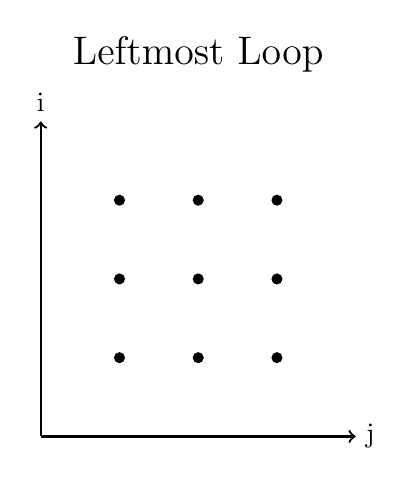
\begin{tikzpicture}
        % Axes
        \draw[->,thick] (0,0) -- (0,4) node[above] {i};
        \draw[->,thick] (0,0) -- (4,0) node[right] {j};
        
        % Grid points
        \foreach \x in {1,2,3}
            \foreach \y in {1,2,3}
                \fill (\x,\y) circle (2pt);
        
        % Title
        \node[above] at (2,4.5) {\Large Leftmost Loop};
    \end{tikzpicture}

    \begin{lstlisting}[language=c]
        //parallel
        for (int i = 0; i < N; i++) {
            A[i][0] = i+1;
        }
    \end{lstlisting}

    for the second loop each iteration of k depends on an earlier iteration of k.

    we have the following system of equations to solve:

    (i1, k1) = (i2, k2-1) which gives us the direction vector [=, <]

    using the theorem from slide 10/37:
    'Th. Parallelism: A loop in a loop nest is parallel iff all its directions
    are either = or there exists an outer loop whose corresp. direction is <'
    
    the outer loop i is parallel, but the inner loop over k, as it has '<' direction and its outer loop does not have a '<' direction, cannot be parallelized.

    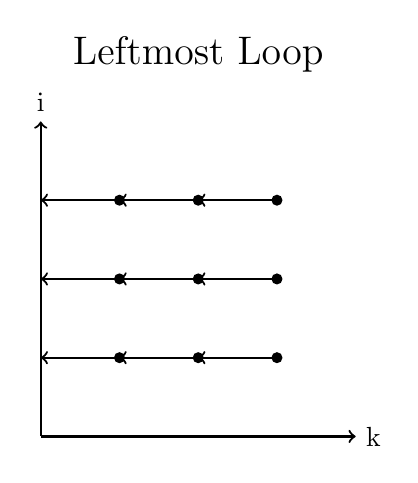
\begin{tikzpicture}
        % Axes
        \draw[->,thick] (0,0) -- (0,4) node[above] {i};
        \draw[->,thick] (0,0) -- (4,0) node[right] {k};

        \draw[<-, thick] (0, 1) -- (1, 1);
        \draw[<-, thick] (1,1) -- (2,1);
        \draw[<-, thick] (2,1) -- (3,1);

        \draw[<-, thick] (0, 2) -- (1, 2);
        \draw[<-, thick] (1,2) -- (2,2);
        \draw[<-, thick] (2,2) -- (3,2);

        \draw[<-, thick] (0, 3) -- (1, 3);
        \draw[<-, thick] (1,3) -- (2,3);
        \draw[<-, thick] (2,3) -- (3,3);
        
        % Grid points
        \foreach \i in {1,2,3}
            \foreach \k in {1,2,3}
                \fill (\i,\k) circle (2pt);
        
        % Title
        \node[above] at (2,4.5) {\Large Leftmost Loop};
    \end{tikzpicture}

    \begin{lstlisting}[language=c]
    //parallel
    for (int i = 0; i < N; i++) {
        // sequential 
        for (int k = 1; k < 2*M; k++) {
            A[i][k] = sqrt(A[i][k-1] * i * k);
        }
    }
    \end{lstlisting}

    for the last loop, we have 

    we have the following system of equations to solve:

    for B
    (i1 + 1, j1 + 1) = (i2, j2) which gives us the direction vector [$<$, $<$]
    for C
    (a1, b1 + 1) = (a2, b2) which gives us the direction vector [=, $<$]
 

    by the same reasoning as for the second loop, the read write to C cannot be parallelized on both levels but only the outer loop.
    B can be parallelized on both levels and thus we could split it up into two

    \begin{lstlisting}[language=c]
    // parallel
    for (int i = 0; i < N; i++) {
        // parallel
        for (int j = 0; j < M; j++) {
            B[i+1, j+1] = B[i, j] * A[i][2*j  ];
        }

        //sequential
        for (int j = 0; j < M; j++) {
            C[i,   j+1] = C[i, j] * A[i][2*j+1];
        }
        
    }
    \end{lstlisting}
    

    \item Explain in terms of direction-vectors why is it legal to apply loop
   interchange on the third (last) loop nest. After interchange, please
   re-analyze the parallelism of the two loops in the third nest; has
   something changed?

    using the theorem from slide 12/37:
    'Th. Loop Interchange: A column permutation of the loops in a loop
    nest is legal iff permuting the direction matrix in the same way does
    NOT result in a > direction as the leftmost non-= direction in a row.'

    as interchange would imply [$<$, $<$] -> [$<$, $<$] for B 
    and [$=$, $<$] -> [$<$, $=$] for C, loop interchange is legal.

    our code now looks like this:

    \begin{lstlisting}[language=c]
    for (int j = 0; j < M; j++) {
        for (int i = 0; i < N; i++) {
            B[i+1, j+1] = B[i, j] * A[i][2*j  ];
            C[i,   j+1] = C[i, j] * A[i][2*j+1];
        }
    }


    Please show the code after interchange and annotate each loop
    with the comment \texttt{// parallel} or \texttt{// sequential}.
\end{itemize}

\section{Task 2: Pen and Paper Exercise Aimed at Recognizing Parallel Operators (3 pts)}

Assume that both A and B are matrices with N rows and 64 columns. Consider the pseudocode below:

\begin{lstlisting}[language=C]
float A[N,64];
float B[N,64];
float accum, tmpA;
for (int i = 0; i < N; i++) { // outer loop
    accum = 0;
    for (int j = 0; j < 64; j++) { // inner loop
        tmpA = A[i, j];
        accum = sqrt(accum) + tmpA*tmpA; // (**)
        B[i,j] = accum;
    }
}
\end{lstlisting}

Reason about the loop-level parallelism of the code above and answer the following in your report:

\begin{enumerate}
    \item Why is the outer loop \textbf{not} parallel? 
    \item Please explain what technique can be used to make it parallel and why is it safe to apply it?
  Re-write the code such that the outer loop is parallel, 
        i.e., the outer loop does not carry any dependencies.
    \item Explain why the inner loop is \textbf{not} parallel.
    \item Assume the line marked with \texttt{(**)} is re-written as \texttt{accum = accum + tmpA*tmpA}.
  Now it is possible to rewrite both the inner and the outer loop as a nested 
    composition of parallel operators! Please write in your report a 
    semantically-equivalent, nested-parallel Futhark program.
\end{enumerate}

\textbf{Clarification:} at step 4. above, we ask you to use human reasoning to
derive a semantically-equivalent program that is fully parallel and is written
in terms of the basic-blocks of functional programming, such as map, reduce, scan, etc. 

\section{Task 3: Histogram-like Computation -- Cuda Exercise 1 (3 pts)}

See section "LL\$ threshing: Histogram-like computation" in companion lecture slides \texttt{L6-locality.pdf}.

The programming task refers to implementing the missing code in files \texttt{main-gpu.cu} and \texttt{kernels.cu.h}---search for keyword "Exercise" in those files and follow the instructions.

Program arguments are, e.g., see Makefile:

\begin{itemize}
    \item The first argument of the program is the size \texttt{N} of the array of indices/values. 
    \item The second argument of the program is the size of the last-level cache (LL\$) in bytes. Please make sure to adjust it to the hardware you are running on (both CPU and GPU), otherwise you will not observe much. The sizes used in the makefile are particularized to the \texttt{hendrixfut01fl} and \texttt{hendrixfut03fl} machines.
    \item The size of the histogram is computed internally such as four passes over the input are always performed.
\end{itemize}

Briefly comment in your report on:

\begin{itemize}
    \item the code implementing your solution, i.e., present
    the code and comment on its correctness and on
    how it optimizes locality. For example, why do
    you expect speedup when the improved implementation
    performs a factor of 3-4x more accesses to global memory
    (since it traverses the input four times).
    \item specify whether your implementation validates
    \item report the GB/sec achieved by your implementations and of the GPU baseline
    and also report the speedup in comparison with the GPU baseline
    (i.e., the other provided implementation)
\end{itemize}

\section{Task 4: Optimizing Spatial Locality by Transposition -- CUDA exercise 2 (4 pts)}

See section "Optimizing Spatial Locality by Transposition" in companion lecture slides \texttt{L6-locality.pdf}.

The programming task refers to implementing in folder \texttt{gpu-coalescing}: 

\begin{enumerate}
    \item In file \texttt{goldeSeq.h}, please \textbf{correctly} parallelize by means of OpenMP the outer loop \texttt{for(uint64\_t i = 0; i < num\_rows; i++) ...}. 
    
    \textbf{Hint:} Task 2 should have taught you what "correctly" means. If the parallel runtime is in the same ballpark as the sequential one, it probably means that it was incorrectly parallelized. (Yes, the incorrect code still validates, can you figure out why?)
    
    \item The code of CUDA kernel \texttt{transKernel} in file \texttt{kernels.cu.h}, which works on the transposed versions of A and B, named \texttt{A\_tr} and \texttt{B\_tr}, respectively. Please search for keyword "Exercise" in file \texttt{kernels.cu.h} to find the implementation place.
\end{enumerate}

Please include in your report:

\begin{itemize}
    \item The OpenMP (parallel) code of \texttt{goldeSeq.h}; report the speedup obtained
   by parallelizing golden sequential, i.e., sequential CPU runtime divided by
   parallel runtime.
    \item the CUDA-kernel code implementing your solution, i.e., present the code and comment on
    its correctness and on how it optimizes spatial locality (i.e., coalesced
    access to global memory). For example, why do
    you expect speedup when \textbf{your} implementation
    performs a factor of 3x more access to global
    memory than the baseline.
    \item specify whether your CUDA implementation validates. (The handin does not, since that kernel is for you to implement).
    \item report the GB/sec achieved by \textbf{your} GPU implementation and of
    the GPU \textbf{baseline} , and also report the speedup w.r.t. the
    baseline.
    \item briefly explain why the CPU implementation that uses GPU-like
  coalescing has abysmal performance (i.e., much slower than the baseline).
    \item \textbf{BONUS} briefly explain at a very high level, why/how
    "the Optimal-GPU Program" is about 2x faster than your implementation.
   ("the Optimal-GPU Program" is the last GPU program run by the Makefile)
\end{itemize}

\section{Task 5: Matrix-Matrix Multiplication (MMM) -- Cuda Exercise 3  (4 pts)}

See section "L1\$ and Register: Matrix-Matrix Multiplication" in companion lecture slides \texttt{L6-locality.pdf}.

The programming task refers to implementing in folder \texttt{mmm} some of the code of Cuda kernel \texttt{mmmSymBlkRegInnSeqKer} in file \texttt{kernels.cu.h}. Please search for keyword "Exercise" in file \texttt{kernels.cu.h} to find the implementation place, and follow the instructions there. Also look around to see how it is called from the CPU (host) code.

Please be aware that Section 6.4 of lecture notes presents a different tiling
strategy for matrix-matrix multiplication; i.e., it is related but it is \textbf{not}
what you have to do.

Briefly comment in your report on:

\begin{itemize}
    \item the code implementing your solution, i.e., show the code and comment on it,
    e.g., explaining why the access to global memory is coalesced
    \item specify whether your implementation validates,
    \item report the performance in Gflops achieved by \textbf{your} GPU implementation
    and by the GPU \textbf{baseline} , and also report the speedup w.r.t. the
    baseline.
    \item Finally, explain in your report the high-level reasons for obtaining
    this speedup, i.e., how did your implementation improved the temporal
    locality (e.g., by what factor has decreased the number of accesses to
    global memory).
\end{itemize}

\section{Task 6: Batched Matrix Multiplication Under a Mask -- Cuda Exercise 4 (4 pts)}

See section "L1\$ and Register: Batch Matrix Multiplication under a Mask" in companion lecture slides \texttt{L6-locality.pdf}.

The programming task refers to implementing in folder \texttt{batch-mmm} the code of the Cuda kernel \texttt{bmmmTiledKer} in file \texttt{kernels.cu.h}. Please search for keyword "Exercise" in file \texttt{kernels.cu.h} to find the implementation place, and follow the instructions there. Remember to flatten the indices to all arrays hold in global memory. Also look around to see how it is called from the CPU (host) code.

Briefly comment in your report on:

\begin{itemize}
    \item the code implementing your solution,
    \item specify whether your implementation validates,
    \item report the performance in Gflops achieved by \textbf{your} GPU implementation
    and by the GPU \textbf{baseline} , and also report the speedup w.r.t. the
    baseline.
    \item Finally, explain in your report the high-level reasons for obtaining
    this speedup, i.e., how did your implementation improved the temporal
    locality (e.g., by what factor has decreased the number of accesses to
    global memory).
\end{itemize}

\end{document}